\documentclass[a4paper, twocolumn]{article}

\usepackage[english]{babel}
\usepackage[utf8]{inputenc}

\usepackage{amssymb, amsmath}
\usepackage{physics}
\usepackage{graphicx, xcolor, subfig,dblfloatfix}
\usepackage{siunitx}
\usepackage{geometry}

\graphicspath{./def_graph/}

%*****RELAZIONE DOMINIO FREQUENZA*****

\begin{document}
\title{Use of Operational Amplifier as  an Integrator and Differentiator}
\author{Stefano Pilosio}

\maketitle
% \begin{multicols}{2}


\section{Abstract}
The objective was to measure the frequency response of two similar circuits, even thought use the same components, show different behaviors, not only in the resulting waveform, but also in the Frequency Response.

\section{Introduction}

\subsection{Operational Amplifier} 

The circuits are made of a resistor ($R$), a capacitor ($C$) and an operational amplifier. To analyze the circuits' behavior it is required to know the feature of an ideal operational amplifier, herein referred as ``OPAMP''.

The ideal OPAMP is a voltage-controlled voltage source, with a voltage gain $E = \frac{V_o}{V_i}$, where $V_o$ is the output voltage and $V_i$ is the input voltage. In this case $V_o$ is referenced to ground, while $V_i$ is the voltage difference between two poles, that are named as inverting ($V^+$) and not inverting ($V^-$) inputs, so $V_i=V^+-V^-$. In the ideal OPAMP $E\to\infty$.

To run the circuit in the desired configuration it is mandatory to use a negative feedback loop, so are respected the condition to use \emph{virtual short circuit principle}. From this principle follows the stability of negative feedback, $E\to\infty$ and $V^+-V^-=0$. From the latter the principle is also named 'Virtual Ground': often the not-inverting input is at ground potential, so $V^+=0=V^-$.

\subsection{Integrator Circuit}
\label{sec:integr}

\begin{figure}
    \centering
    \def\svgwidht{\columnwidth}
    \input{def_graph/IntegratorCircuit.pdf_tex}
    \caption{Schematic of an Integrator Circuit}
    \label{fig:IntegrScheme}
\end{figure}

Referring to Figure~\ref{fig:IntegrScheme}, in the negative feedback loop there is a capacitor and a resistor.
Using Ohm's Law, Capacitor Law ($ q = Cv \implies \dv {q}{t}=i=C\dv{v}{t} $) and KCL it is obtained:
\begin{gather*}
    \begin{cases}
        v_{IN} - R\cdot i_R = v^-\\
        i_R=i_C\\
        v^+-v^-=0\\
        v^+=0\\
        i_C=C\dv{v^--v_{OUT}}{t}
    \end{cases}\\
    i = \frac{v_{IN}}{R}=-C\dv{v_{OUT}}{t}\\
\end{gather*}

From last equation, resolving for $v_{OUT}$:

\begin{equation}
    \label{eq:Integrator}
    v_{OUT}=-\frac{1}{CR}\int_0^t{v_{IN}}\,dt + v(0)
\end{equation}

It is visible from~\eqref{eq:Integrator}, that the behavior of this circuit in time domain is to produce the input voltage integral function.

The frequency response is defined as \[H=\frac{v_{OUT}}{v_{IN}}(f)\].
To obtain $H(f)$, it is applied Fourier Transform (FT) over \eqref{eq:Integrator}:

\begin{gather}
    V_{OUT}=-\frac{1}{CR(j2\pi f)}V_{IN}\\
    H = \frac{V_{OUT}}{V_{IN}} = \frac{1}{RC(j2\pi f)}   
\end{gather}

\begin{center}
    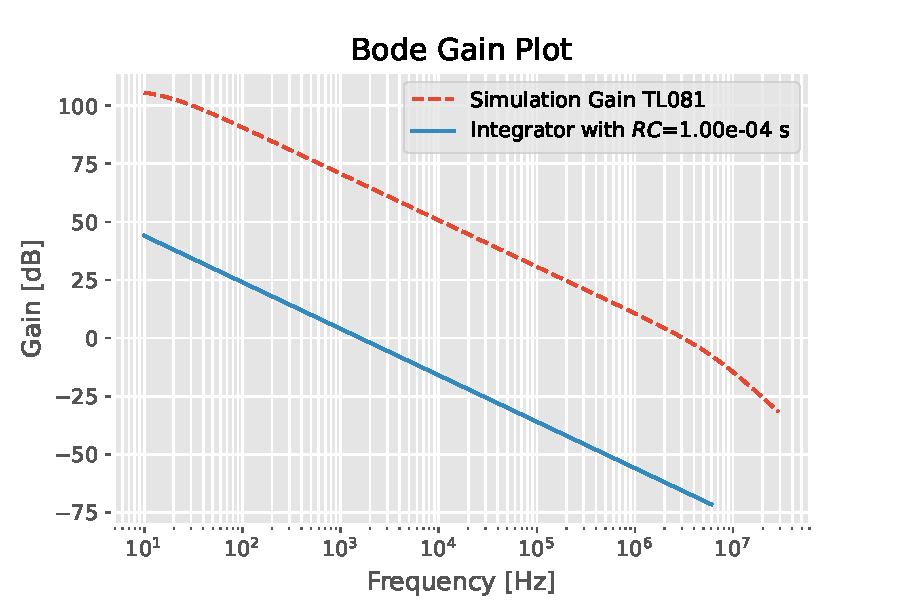
\includegraphics[width=\columnwidth]{def_graph/IntegratorBodeTheo.pdf}
    \label{fig:IntBodeGraphTheo}
\end{center}

The Bode Gain Diagram in Figure~\ref{fig:IntBodeGraphTheo}shows a constant negative monotony of \SI{-20}{\deci\bel/Dec}, it means the output attenuation is increasing with the frequency.

In the diagram is also shown the open loop gain of the OPAMP, that shows the real behavior of the OPAMP. The OPAMP has much higher gain than what permits the frequency response of the circuit, so the OPAMP never outputs its max gain at any frequency, this is due to the negative feedback loop that limits the circuit gain in a dynamical way compared to a resistive voltage divider which statically limits the gain.

\subsection{Differentiator Circuit} 
\label{sec:diff}

\begin{figure}
    \centering
    \def \svgwidht{\columnwidth}
    \input{def_graph/DifferentiatorCircuit.pdf_tex}
    \caption{Schematic of a Differentiator Circuit}
    \label{fig:DifferScheme}
\end{figure}

As shown in Figure~\ref{fig:DifferScheme}, the circuit is similar to the previous case, but in this case the capacitor and the resistor are swapped. This change produces a completely different response to the input waveform, it can be understood writing KCL, the Ohm's Law and the capacitor law.

\begin{gather*}
    \begin{cases}
        i_C = C\dv{v_{IN}-v^-}{t}\\
        i_R = \frac{v^--v_{OUT}}{R}\\
        i_R = i_C\\
        v^+=v^-\\
        v^-=0
    \end{cases}
    C\dv{v_{IN}}{t}=\frac{-v_{OUT}}{R}
\end{gather*}

As in the precedent case resolving for $v_{OUT}$
\begin{equation}
    \label{eq:Differentiator}
    v_{OUT}=RC\dv{v_{IN}}{t}
\end{equation}

\eqref{eq:Differentiator} shows that $v_{OUT}$ is a waveform proportional to the derivative of the input waveform. 

Calculating \(H\) produces:
\begin{gather}
    V_{OUT}=RC\cdot(j2\pi f)V_{IN}\\
    H = RC\cdot(j2\pi f)
\end{gather}

\begin{center}
    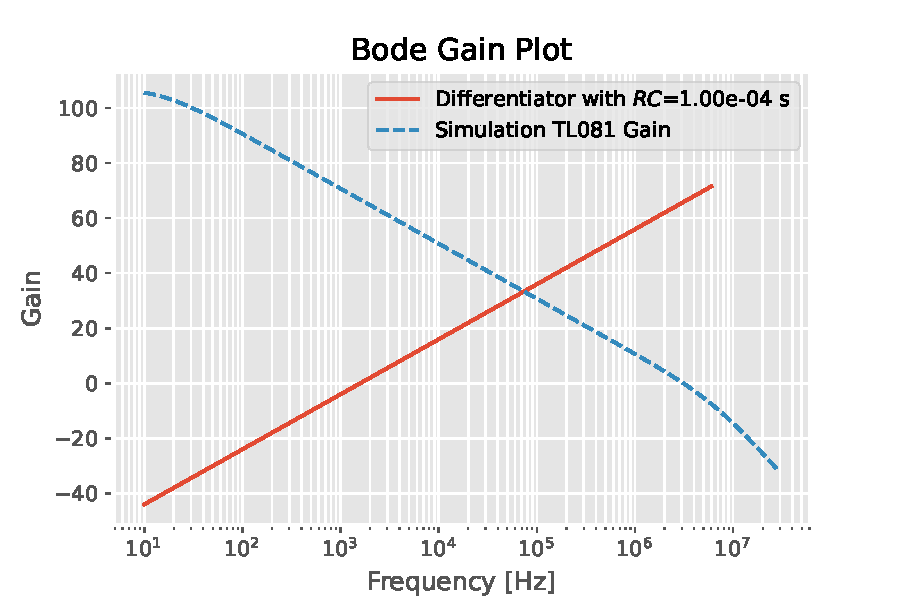
\includegraphics[width=\columnwidth]{def_graph/DifferentiatorBodeTheo.pdf}
    \label{fig:DiffBodeGraphTheo}
\end{center}

In this case the circuit has a constant positive monotony of 20 dB/Dec, so output signal amplification is directly related to the frequency. In this case we can expect a peak at the frequency in the point where the open loop OPAMP gain intersects the circuit frequency response, then the behavior of the circuit will be similar to the open loop OPAMP due to the limitation of a real OPAMP.

Also in this circuit we can see a dynamic change in the output gain of the circuit but with the opposite behavior of the precedent cases, but it is limited to what can supply the OPAMP. This leads to the conclusion that with a more complex feedback loop it is possible to amplify only some chosen frequency with the high gain that produces an OPAMP or to modulate the frequency response on some desired function, maybe with the right condition it is possible to produce periodical signal without an input signal.

\section{Measurement Methods}

% Sottosezone strumenti di misura
\subsection{Materials}
\subsubsection{Instruments}
\begin{itemize}
    \item Oscilloscope ``Tektronix TDS 1012B'';
    \item Function Generator ``Agilent 3322A'';
    \item Power Supply.
\end{itemize}
\subsubsection{Equipment}
\begin{itemize}
    \item OPAMP ``LT081'';
    \item Breadboard;
    \item Wires;
    \item Resistor (value : \SI{10}{\kilo\ohm}, tolerance : 1\%);
    \item Capacitor (value : \SI{10}{\nano\farad});
\end{itemize}

\subsection{Procedure}

The two circuits are built as shown in the previous Figures \ref{fig:DifferScheme} and \ref{fig:IntegrScheme}, the Oscilloscope probe was connected in the point named \(V_{OUT}\), grounded to ground. The function generator was connected to \(V_{IN}\) and ground.   The OPAMP was powered by a dual power supply, supplying the necessary \(V_{CC+}\) and \(V_{CC-}\).

The measure procedure was:
\begin{enumerate}
    \item Choosing a frequency for the sine wave on the function generator;
    \item Using the oscilloscope it was measured the voltage peak to peak of the input and the output signal;
    \item Then was used the cursor mode on oscilloscope to measure the shift in the peak of the input and the output to obtain the phase, for this the cursor was set on time domain and moved in correspondence of a peak of the input waveform and the nearest peak of the output waveform, at the measure was assigned a positive sign if the output is to the right of input, negative if the output is to the left of input. 
\end{enumerate}

The frequencies have been chosen to use an approximate log scale (like 1, 2, 3, 5, 8, 10). 

\section{Analysis}

\subsection{Computation}

During the measuring process data were saved on a comma separated value text file (CSV). Data have been analyzed using a Python environment with ``\emph{NumPy, Pandas and Matplotlib}'' libraries. This environment was included in a Jupyter Notebook to visualize the analysis results in real time. The code computed and plotted from the data the Bode Diagram and the Nyquist Diagram. Using another software, ``\emph{NGSpice}'', it was simulated the expected behavior in frequency, in the simulation is added a \SI{50}{\ohm} resistor to mimic the function generator impedance. At last data from experiment and simulation are compared in the Python environment.
    
% \end{multicols}

\subsection{Integrator}
\begin{figure*}[ht!]
    \centering
    \subfloat{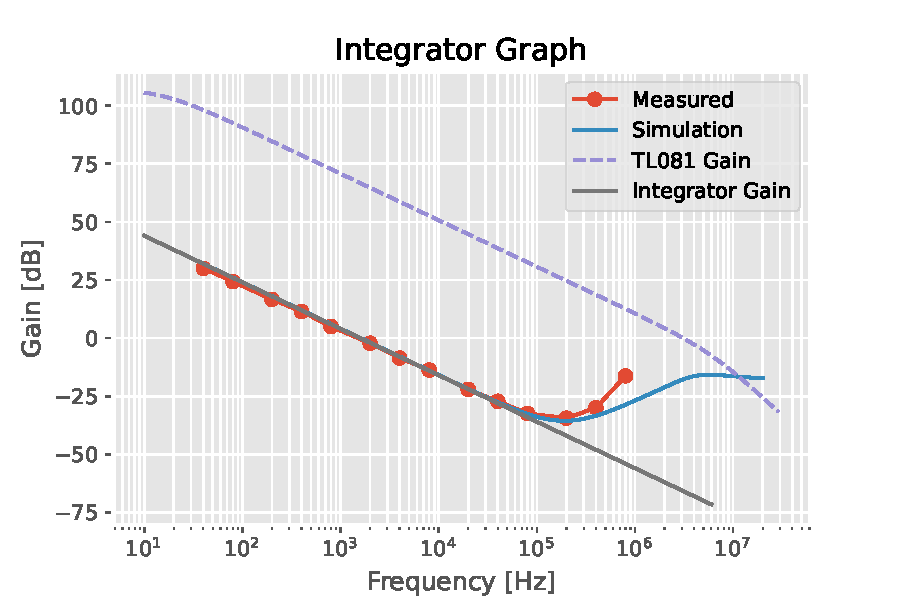
\includegraphics[width = \textwidth]{def_graph/Exp_Integ_graph.pdf}} \\
    \subfloat{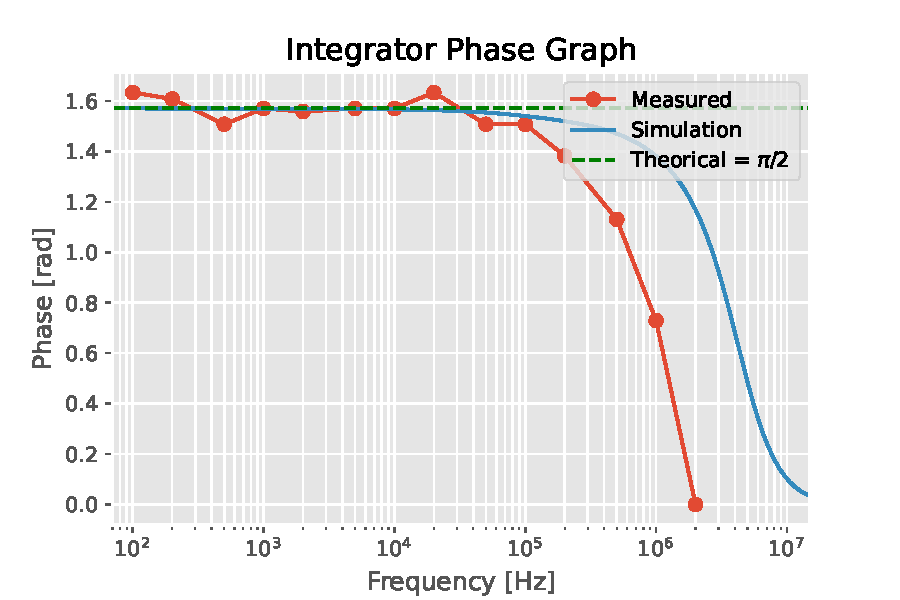
\includegraphics[width = \columnwidth]{def_graph/Exp_Integ_Phase.pdf}} 
    \subfloat{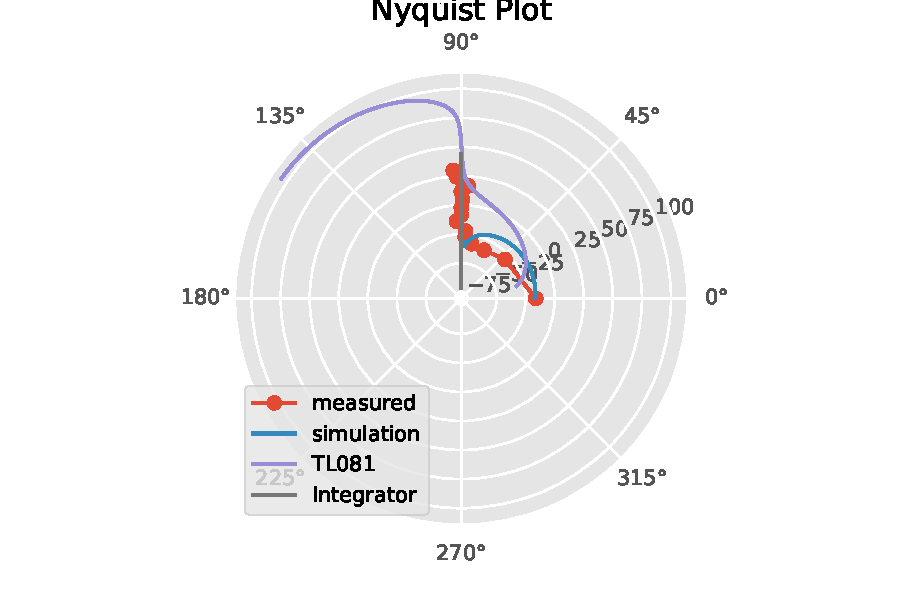
\includegraphics[width = \columnwidth]{def_graph/Exp_Integ_Nyquist.pdf}}
    \caption{Resulting plot after experiment and simulation, it is notable that the frequency response resemble closely the simulated behavior and the expected behavior from section~\ref{sec:integr}.}
    \label{fig:expIntegr}
\end{figure*}

% \begin{multicols}{2}

As shown in Figure~\ref{fig:expIntegr} the frequency response is very similar to the expected one. There is a difference in the curl at high frequency, this is probably due to non-ideal aspect of OPAMP amplification frequency response due to the fact that is present also in the simulation, even so it is not to exclude some breadboard parasitic capacitance, that could have caused some deviation from simulation in the experimental data. The breadboard adds some capacitance, in the order of \unit{\pico\farad}, and some resistance, that influences the response of the circuit. There is an intrinsic difficulty in the manual measure of a low voltage at high frequency, due to signal stability and external electromagnetic effects (Radio waves). The phase graph reinforces the suspect of a parasitic capacitance, in fact the phase change starts at a lower frequency than expected, that is compatible to a higher capacitance.

% \end{multicols}
\subsection{Differentiator}

\begin{figure*} [ht!]
    \centering
    \subfloat{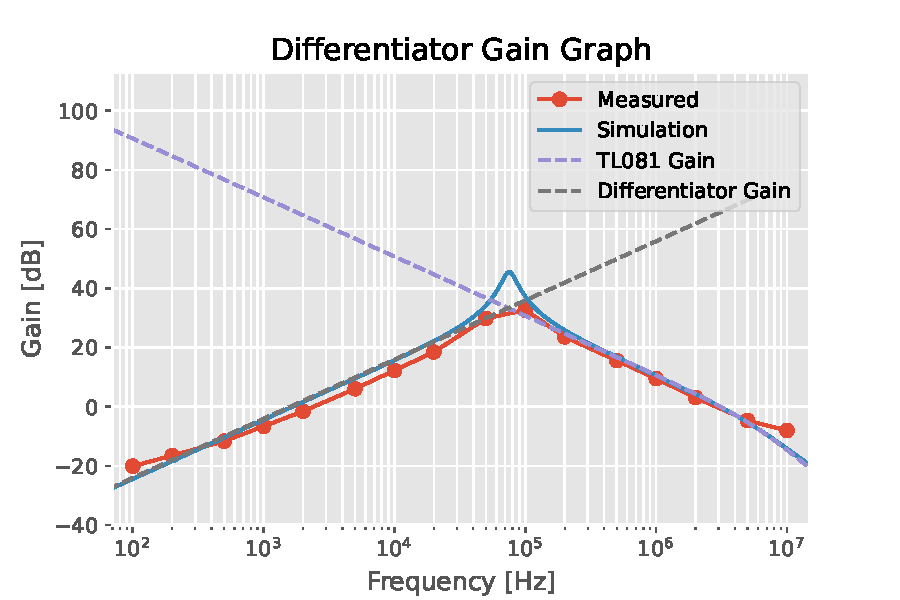
\includegraphics[width = \textwidth]{def_graph/Exp_Diff_graph.pdf}}\\
    \subfloat{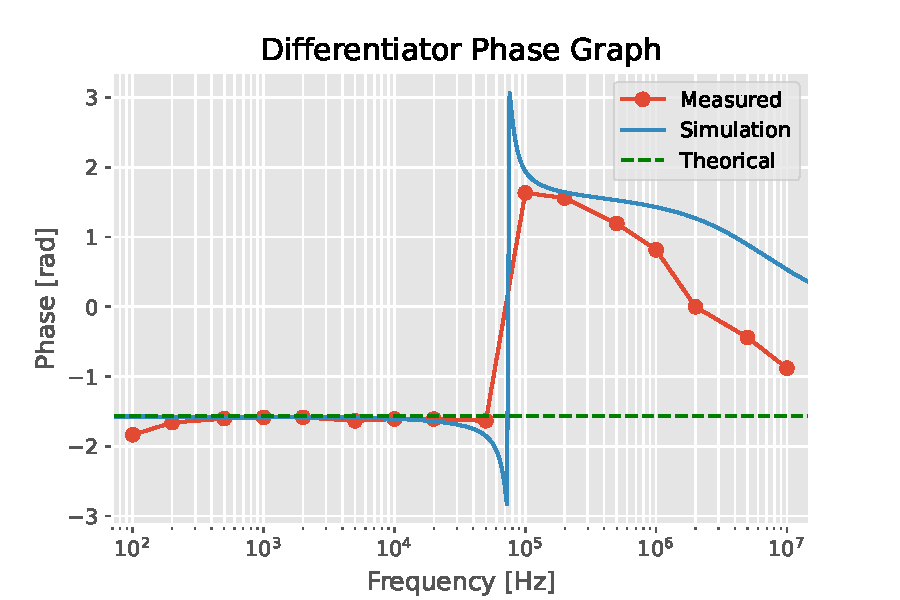
\includegraphics[width = \columnwidth]{def_graph/Exp_Diff_Phase.pdf}} 
    \subfloat{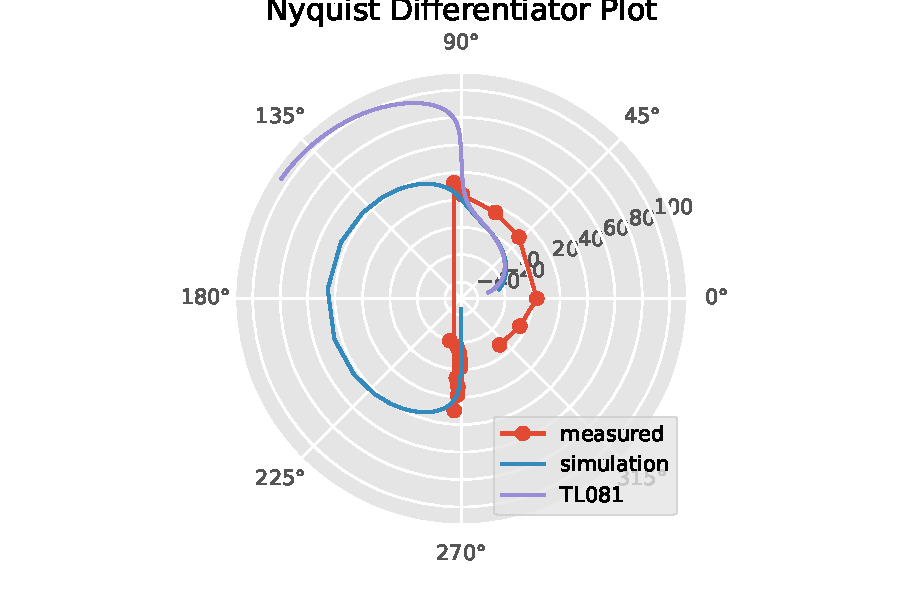
\includegraphics[width = \columnwidth]{def_graph/Exp_Diff_Nyquist.pdf}}
    \caption{Resulting plot after experiment and simulation, it is notable that the frequency response resemble closely what expected in section~\ref{sec:diff}.}
    \label{fig:expDiff}
\end{figure*}

% \begin{multicols}{2}


As shown in Figure~\ref{fig:expDiff} we have a resonance peak at around \SI{75}{\kilo\hertz}, also in this case the experimental trend resembles the simulated very closely. The lack of points around the resonance frequency is due to the used frequency sequence.

In the phase Diagram and also in Nyquist plot is clearly visible when the behavior of the circuit changes from the Differentiator to a classical OPAMP. Even in the case of the Differentiator there is a difficulty in measuring the change in phase due to signal stability.

\section{Conclusion}

At the end we have two interesting circuits that can calculate in real time two complex linear operations such as the derivative and integral of a function, it is interesting also to opposite behavior in respect to the frequency of the circuits and its possible application.  
% \end{multicols}
\end{document}